\documentclass[a4paper,12pt]{article}

%%% Работа с русским языком

\usepackage{cmap}					% поиск в PDF
\usepackage{mathtext} 				% русские буквы в формулах
\usepackage[T2A]{fontenc}			% кодировка
\usepackage[utf8]{inputenc}			% кодировка исходного текста
\usepackage[english,russian]{babel}	% локализация и переносы
\usepackage{indentfirst}            % красная строка в первом абзаце
\usepackage[unicode]{hyperref}
\usepackage{epigraph}
\frenchspacing                      % равные пробелы между словами и предложениями

%%% Дополнительная работа с математикой
\usepackage{amsmath,amsfonts,amssymb,amsthm,mathtools} % пакеты AMS
\usepackage{bbm} % Blackboard bold для цифр
\usepackage{icomma}                                    % "Умная" запятая

\renewcommand{\phi}{\ensuremath{\varphi}}
\renewcommand{\kappa}{\ensuremath{\varkappa}}
\renewcommand{\le}{\ensuremath{\leqslant}}
\renewcommand{\leq}{\ensuremath{\leqslant}}
\renewcommand{\ge}{\ensuremath{\geqslant}}
\renewcommand{\geq}{\ensuremath{\geqslant}}
\renewcommand{\emptyset}{\ensuremath{\varnothing}}

\newcommand{\cl}{\text{cl }}
\newcommand{\setint}{\text{int }}
\newcommand\independent{\protect\mathpalette{\protect\independenT}{\perp}}
\def\independenT#1#2{\mathrel{\rlap{$#1#2$}\mkern2mu{#1#2}}}

\theoremstyle{plain}
\newtheorem{theorem}{Теорема}[section]
\newtheorem{lemma}{Лемма}[section]
\newtheorem{proposition}{Утверждение}[section]
\newtheorem*{corollary}{Следствие}
\newtheorem*{exercise}{Упражнение}

\theoremstyle{definition}
\newtheorem{definition}{Определение}[section]
\newtheorem*{note}{Замечание}
\newtheorem*{reminder}{Напоминание}
\newtheorem*{example}{Пример}
\newtheorem*{tasks}{Вопросы и задачи}

\theoremstyle{remark}
\newtheorem*{solution}{Решение}

%%% Оформление страницы
\usepackage{extsizes}     % Возможность сделать 14-й шрифт
\usepackage{geometry}     % Простой способ задавать поля
\usepackage{setspace}     % Интерлиньяж
\usepackage{enumitem}     % Настройка окружений itemize и enumerate
\usepackage{epigraph}     % Эпиграф
\setlist{leftmargin=25pt} % Отступы в itemize и enumerate

\geometry{top=25mm}    % Поля сверху страницы
\geometry{bottom=30mm} % Поля снизу страницы
\geometry{left=20mm}   % Поля слева страницы
\geometry{right=20mm}  % Поля справа страницы

\begin{document}
\tableofcontents
\newpage

\section{Базовые определения}

\begin{definition}
	Система $\mathcal{F}$ подмножеств $\Omega$ называется алгеброй, если
	\begin{enumerate}
		\item $\Omega \in \mathcal{F}$
		\item $A \in \mathcal{F}$, то $\overline{A} := (\Omega \setminus A) \in \mathcal{F}$
		\item $A,\, B \in \mathcal{F}$, то $A \cap B \in \mathcal{F}$
	\end{enumerate}
\end{definition}

\begin{definition}
	Система $\mathcal{F}$ подмножеств $\Omega$ называется $\sigma$-алгеброй, если
	\begin{enumerate}
		\item $\mathcal{F}$ -- алгебра
		\item $\forall \{A_n,\, n \in \mathbb{N}\},\, A_n \in \mathcal{F} \Rightarrow \cup_{n = 1}^\infty A_n \in \mathcal{F}$
	\end{enumerate}
\end{definition}

\begin{definition}
	$P$ называется вероятностной мерой на $(\Omega,\, \mathcal{F})$, если $P:\: \mathcal{F} \to [0,\,1]$, удовлетворяющая свойствам:
	\begin{enumerate}
		\item $P(\Omega) = 1$
		\item Если $\{A_n,\, n \in \mathbb{N}\}$, то
		      \[P\left(\bigsqcup_{n = 1}^\infty A_n\right) = \sum_{n = 1}^\infty P(A_n)\]
	\end{enumerate}
\end{definition}

\begin{definition}
	Вероятностное пространство -- это тройка $(\Omega,\, \mathcal{F},\, P)$, где
	\begin{itemize}
		\item $\Omega$ -- множество элементарных исходов
		\item $\mathcal{F}$ -- $\sigma$-алгебра подмножеств $\Omega$, элементы $\mathcal{F}$ называются событиями
		\item $P$ -- вероятностная мера на измеримом пространстве $(\Omega,\, \mathcal{F})$
	\end{itemize}
\end{definition}

\begin{definition}
	Система $\mathcal{M}$ подмножеств в $\Omega$ называется $\pi$-системой, если из того, что $A,\, B \in \mathcal{M}$ следует, что $A \cap B \in \mathcal{M}$
\end{definition}

\begin{definition}
	Система $\mathcal{L}$ подмножеств в $\Omega$ называется $\lambda$-системой, если
	\begin{enumerate}
		\item $\Omega \in \mathcal{L}$
		\item $(A,\, B \in \mathcal{L};\; A \subset B) \Rightarrow B \setminus A \in \mathcal{L}$
		\item $(A_n \uparrow A;\; \forall n \: A_n \in \mathcal{L}) \Rightarrow A \in \mathcal{L}$
	\end{enumerate}
\end{definition}

\begin{theorem} \label{FIRST_SYSTEM_TH}
	Первая теорема о $\pi$-$\lambda$-системах

	Система $\mathcal{F}$ подмножеств $\Omega$ является $\sigma$-алгеброй $\Leftrightarrow$ она является $\pi$-системой и $\lambda$-системой.
\end{theorem}

\begin{proof}
	$\Rightarrow$ очевидно.

	$\Leftarrow$ Проверим сначала, что $\mathcal{F}$ -- алгебра. Свойства $1),\,2)$ уже есть. По свойству $2)$ $\lambda$-системы $\overline{A} = \Omega \setminus A \in \mathcal{F}$, если $A \in \mathcal{F}$. Значит $\mathcal{F}$ -- алгебра.

	Пусть $\{A_n,\, n \in \mathbb{N}\},\, \forall n \: A_n \in \mathcal{F},\, \forall i \neq j \: A_i \cap A_j = \emptyset$. Рассмотрим $B_n = \sqcup_{m = 1}^n A_m \in \mathcal{F}$. Тогда $B_n \subset B_{n + 1}$ и $\cup_{n = 1}^\infty B_n = \sqcup_{n = 1}^\infty A_n \Rightarrow$ по $3)$ свойству $\lambda$-системы: $B_n \uparrow \sqcup_{n = 1}^\infty A_n \in \mathcal{F}$.
\end{proof}

\begin{lemma}
	Пусть $\mathcal{M}$ -- система подмножеств $\Omega$. Тогда существует минимальная (по включению) $\sigma$-алгебра (алгебра, $\pi$-система, $\lambda$-система), обозначаемая $\sigma(\mathcal{M})$ ($\lambda(\mathcal{M}),\, \pi(\mathcal{M}),\, \lambda(\mathcal{M})$), содержащая $\mathcal{M}$.
\end{lemma}

\begin{example}
	\begin{enumerate}
		\item Если $\Omega = \mathbb{R}$, то борелевской $\sigma$-алгеброй на $\mathbb{R}$ называется наименьшая $\sigma$-алгебра, содержащая все интервалы
		      \[\mathcal{B}(\mathbb{R}) = \sigma((a;\;b) ,\: a < b)\]
		\item Если $\Omega = \mathbb{R}^n,\, n > 1$.

		      Борелевской $\sigma$-алгеброй в $\mathbb{R}^n$ называется минимальная $\sigma$-алгебра, содержащая множества вида $B_1 \times \cdots \times B_n,\, B_i \in \mathcal{B}(\mathbb{R})$, то есть
		      \[\mathcal{B}(\mathbb{R}^n) = \sigma(B_1 \times \cdots \times B_n:\: B_i \in \mathcal{B}(\mathbb{R}))\]
		\item Если $\Omega = \mathbb{R}^\infty$, то есть $\Omega$ содержит все счётные последовательности вещественных чисел.

		      Для $n \in \mathbb{N}$ и $B_n \in \mathcal{B}(\mathbb{R}^n)$ введём циллиндр:
		      \[F_n(B_n) = \{\vec{x} \in \mathbb{R}^\infty :\: (x_1,\,\cdots,\,x_n) \in B_n\}\]
		      Тогда минимальная $\sigma$-алгеьра, содержащая все циллиндры называется борелевской в $\mathbb{R}^\infty$, то есть
		      \[\mathcal{B}(\mathbb{R}^\infty) = \sigma(F_n(B_n):\: n \in \mathbb{N},\, B_n \in \mathcal{B}(\mathbb{R}^n))\]
	\end{enumerate}
\end{example}

\section{Вторая теорема о $\pi$- и $\lambda$-системах. Следствия из неё.}
\begin{theorem} \label{SECOND_SYSTEM_TH}
	Вторая теорема о $\pi$-$\lambda$-системах.

	Если $\mathcal{M}$ -- это $\pi$-система подмножеств в $\Omega$, то $\sigma(\mathcal{M}) = \lambda(\mathcal{M})$
\end{theorem}

\begin{proof}
	Заметим, что $\sigma(\mathcal{M})$ -- $\lambda$-система, содержащая $\mathcal{M} \Rightarrow \lambda(\mathcal{M}) \subset \sigma(\mathcal{M})$.

	Проверим, что $\lambda(\mathcal{M})$ -- это $\sigma$-алгебра. Раз $\lambda(\mathcal{M})$ -- это $\lambda$-система, то по (\ref{FIRST_SYSTEM_TH}) достаточно проверить, что $\lambda(\mathcal{M})$ -- это $\pi$-система.

	Рассмотрим $\mathcal{M}_1 = \{B \in \lambda(\mathcal{M}):\: \forall A \in \mathcal{M},\, A \cap B \in \lambda(\mathcal{M})\}$. Заметим, что $\mathcal{M} \subset \mathcal{M}_1$. Проверим, что $\mathcal{M}_1$ -- это $\lambda$-система:
	\begin{enumerate}
		\item $\Omega \in \mathcal{M}_1$ -- очевидно
		\item Пусть $B,\, C \in \mathcal{M}_1,\, C \subset B$, пусть $A \in \mathcal{M}$. Заметим, что $B \setminus C \in \lambda(\mathcal{M})$ и
		      \[(B \setminus C) \cap A = \stackrel{\in \lambda(\mathcal{M})}{(B \cap A)} \setminus \stackrel{\in \lambda(\mathcal{M})}{(C \cap A)}\]
		      Значит по второму свойству $\lambda$-систем $(B \setminus C) \cap A \in \lambda(\mathcal{M})$
		\item Пусть $B_n \uparrow B,\, B_n \in \mathcal{M}_1,\, A \in \mathcal{M} \Rightarrow$
		      \[\stackrel{\in \lambda(\mathcal{M})}{B_n \cap A}\: \uparrow B \cap A\]
		      Тогда по третьем свойству $\lambda$-систем $B \cap A \in \lambda(\mathcal{M})$. Но $B_n \in \lambda(\mathcal{M}) \Rightarrow$ по третьему свойству $\lambda$-системы получаем, что $B \in \lambda(\mathcal{M}) \Rightarrow B \in \mathcal{M}_1$.
	\end{enumerate}
	По условию $\mathcal{M} \subset \mathcal{M}_1 \Rightarrow$ в силу минимальности $\lambda(\mathcal{M}) \subset \mathcal{M}_1$. По построению $\mathcal{M}_1 \subset \lambda(\mathcal{M}) \Rightarrow \lambda(\mathcal{M}) = \mathcal{M}_1$, то есть $\forall B \in \lambda(\mathcal{M}) \: \forall A \in \mathcal{M} :\: A \cap B \in \lambda(\mathcal{M})$.

	Далее рассмотрим $\mathcal{M}_2 = \{B \in \lambda(\mathcal{M}):\: \forall A \in \lambda(\mathcal{M}) \: A \cap B \in \lambda(\mathcal{M})\}$. В силу доказанного $\mathcal{M} \subset \mathcal{M}_2$. Совершенно аналогично с $\mathcal{M}_1$ проверяем, что $\mathcal{M}_2$ -- это $\lambda$-система. Тогда $\lambda(\mathcal{M}) \subset \mathcal{M}_2$. По построению $\mathcal{M}_2 \subset \lambda(\mathcal{M}) \Rightarrow \lambda(\mathcal{M}) = \mathcal{M}_2 \Rightarrow \lambda(\mathcal{M})$ -- это $\pi$-система.
\end{proof}

\begin{corollary}
	Пусть $\mathcal{M}$ -- это $\pi$-система на $\Omega$, и $\mathcal{L}$ -- это $\lambda$-система на $\Omega$ и $\mathcal{M} \subset \mathcal{L}$. Тогда $\lambda(\mathcal{M}) \subset \mathcal{L}$
\end{corollary}

\section{Независимость событий и систем событий}
\begin{definition}
	События $A,\, B$ независимые, если
	\[P(A \cap B) = P(A) \cdot P(B)\]
\end{definition}

\begin{definition}
	События $A_1,\,\cdots,\,A_n$ называются независимыми в совокупности, если \[\forall k \leq n \: \forall 1 \leq i_1 < \cdots < i_k \leq n :\: P\left(\bigcap_{j = 1}^k A_{i_j}\right) = \prod_{j = 1}^k P(A_{i_k}) \]
\end{definition}

\begin{definition}
	Пусть $\mathcal{M}_1,\,\cdots,\,\mathcal{M}_n$ -- системы событий на $(\Omega,\, \mathcal{F},\, P)$. Они называются независимыми в совокупности, если
	\[\forall A_1 \in \mathcal{M}_1,\, \cdots,\, A_n \in \mathcal{M}_n:\: A_1,\,\cdots,\,A_n - \text{ независимы в совокупности}\]
\end{definition}

\begin{lemma} \label{INDEPENDENCE_CRIT}
	Критерий независимости $\sigma$-алгебр.

	Пусть $\mathcal{M}_1,\,\cdots,\,\mathcal{M}_n$ -- это $\pi$-системы событий на $(\Omega,\, \mathcal{F},\,P)$. Тогда $\mathcal{M}_1,\,\cdots,\,\mathcal{M}_n$ -- независимы в совокупности $\Leftrightarrow \sigma(\mathcal{M}_1),\,\cdots,\,\sigma(\mathcal{M}_n)$ -- независимы в совокупности.
\end{lemma}

\begin{proof}
	$\Leftarrow$ очевидно.

	Докажем только для $n = 2$, для $n > 2$ всё аналогично.

	Рассмотрим $\mathcal{L}_1 = \{A \in \sigma(\mathcal{M}_2):\: A \independent \mathcal{M}_1\}$. Проверим, что $\mathcal{L}_1$ -- это $\lambda$-система:
	\begin{enumerate}
		\item $\forall B \in \mathcal{M}_1 :\: \Omega \independent B \Rightarrow \Omega \in \mathcal{L}_1$
		\item Пусть $C \in \mathcal{M}_1$, тогда
		      \begin{align*}
			      P((B \setminus A) \cap C) = P((B \cap C) \setminus (A \cap C)) = P(B \cap C) - P(A \cap C) = \\
			      P(C)(P(B) - P(A)) = P(B \setminus A)P(C) \Rightarrow B \setminus A \in \mathcal{L}_1
		      \end{align*}
		\item Пусть $A_n \uparrow A,\, A_n \in \mathcal{L}_1$. По определению $\sigma$-алгебры замечаем, что $A \in \sigma(\mathcal{M}_2)$. Пусть $C \in \mathcal{M}_1$. Рассмотрим
		      \[P(A \cap C) = \lim_{n \to +\infty} P(A_n \cap C) = P(C)\lim_{n \to +\infty}P(A_n) = P(C)P(A) \Rightarrow A \in \mathcal{L}_1\]
	\end{enumerate}
	Раз $\mathcal{L}_1$ -- это $\lambda$-система и $\mathcal{M}_2 \subset \mathcal{L}_1$, по условию, то по (\ref{SECOND_SYSTEM_TH}) получим, что $\sigma(\mathcal{M}_2) \subset \mathcal{L}_1 \Rightarrow \sigma(\mathcal{M}_2) \independent \mathcal{M}_1$.

	Рассмотрим $\mathcal{L}_2 = \{A \in \sigma(\mathcal{M}_1):\: A \independent \sigma(\mathcal{M}_2)\}$. Точно так же доказывается, что $\mathcal{L}_2$ -- это $\lambda$-система, $\mathcal{M}_1 \subset \mathcal{L}_2$ по доказанному $\Rightarrow \sigma(\mathcal{M}_1) \subset \mathcal{L}_2 \Rightarrow \sigma(M_1) \independent \sigma(M_2)$
\end{proof}

\begin{definition}
	Пусть $\{M_\alpha,\, \alpha \in \mathfrak{A}\}$ -- набор систем событий. Он называется независимым в совокупности, если независим в совокупности $\forall$ конечный поднабор.
\end{definition}

\section{Функция распределения вероятностной меры}
\begin{definition}
	Функцией распределения вероятностной меры $P$ на $\mathbb{R}$ называется
	\[F(x) = P((-\infty,\, x]),\, x \in \mathbb{R}\]
\end{definition}

\begin{lemma}
	Свойства функции распределения.

	\begin{enumerate}
		\item $F(x)$ не убывает
		\item $F(+\infty) = 1,\, F(-\infty) = 0$
		\item $F(x)$ непрерывна справа
	\end{enumerate}
\end{lemma}

\begin{proof}
	\begin{enumerate}
		\item Пусть $y > x$. Тогда
		      \[(-\infty,\, x] \subset (-\infty,\, y] \Rightarrow F(x) = P((-\infty,\, x]) \leq P((-\infty,\, y]) = F(y)\]
		\item Если $x_n \uparrow +\infty$, то $(-\infty,\, x_n] \uparrow \mathbb{R}$. Тогда в силу непрерывности меры
		      \[F(x_n) = P((-\infty,\, x_n]) \stackrel{n \to +\infty}{\to} P(\mathbb{R}) = 1\]
		      Если $x_n \downarrow -\infty$, то $(-\infty,\, x_n] \downarrow \emptyset$. Тогда в силу непрерывности меры
		      \[F(x_n) = P((-\infty,\, x_n]) \stackrel{n \to +\infty}{\to} P(\emptyset) = 0\]
		\item Если $x_n \downarrow x$, то $(-\infty,\, x_n] \downarrow (-\infty,\, x]$. Тогда в силу непрерывности меры
		      \[F(x_n) = P((-\infty,\, x_n]) \stackrel{n \to +\infty}{\to} P((-\infty,\, x]) = F(x)\]
	\end{enumerate}
\end{proof}

\begin{definition}
	Эквивалентное определение функции распределения.

	Функция, удовлетворяющая свойствам $1-3$ из предыдущей леммы, называется функцией распределения на $P$.
\end{definition}

\begin{theorem} \label{MEASURE_EXTEND_TH}
	О продолжении меры (б/д)

	Пусть $\mathcal{A}$ -- алгебра подмножеств $\Omega$. Пусть $P_0 :\: \mathcal{A} \to [0,\,1]$ с условием, $P_0(\Omega) = 1$ и $P_0$ счётно-аддитивна на $\mathcal{A}$. Тогда $\exists!$ продолжение меры $P_0$ на $\sigma(A)$
\end{theorem}

\begin{theorem}
	О взаимной однозначности функции распределения и вероятностной меры.

	Пусть $F(x),\, x \in \mathbb{R}$ -- функция распределения на $\mathbb{R}$. Тогда $\exists!$ вероятностная мера $P$ на $(\mathbb{R},\, \mathcal{B}(\mathbb{R}))$, для которой $F$ является функцией распределения, то есть
	\[\forall x \in \mathbb{R} :\: F(x) = P((-\infty,\,x])\]
\end{theorem}

\begin{proof}
	Рассмотрим на $\mathbb{R}$ алгебру $\mathcal{A}$, состоящую из конечных объединений непересекающихся интервалов:
	\[\forall A \in \mathcal{A}:\: A = \bigsqcup_{k = 1}^n (a_k,\,b_k],\, -\infty \leq a_1 < b_1 < a_2 < b_2 < \cdots < b_n \leq +\infty\]
	Зададим на $\mathcal{A}$ меру $P_0$:
	\[\forall A \in \mathcal{A}:\: P_0(A) = \sum_{k = 1}^n (F(b_k) - F(a_k))\]
	где $F(-\infty) = 0,\, F(+\infty) = 1$.

	По построению $P_0(\mathbb{R}) = 1$ и $P_0$ будет конечно аддитивна на $\mathcal{A}$. Если мы проверим, что $P_0$ счётно аддитивна на $\mathcal{A}$, то по (\ref{MEASURE_EXTEND_TH}) $\exists!$ продолжение $P$ меры $P_0$ на $\sigma(A) = \mathcal{B}(\mathbb{R})$. Это и есть искомая мера $P$, причём
	\[P((-\infty,\, x]) = P_0((-\infty,\, x]) = F(x)\]
	По теореме о непрерывности вероятностной меры, достаточно проверить, что $P_0$ непрерывна в нуле.

	Пусть $A_n \downarrow \emptyset,\, \forall n :\: A_n \in \mathcal{A}$. Хотим проверить, что $P(A_n) \stackrel{n \to +\infty}{\to} 0$. В силу $2-3$ свойств функции распределения:
	\[\forall A \in \mathcal{A} \: \forall \varepsilon > 0 \: \exists B \in A :\: \cl B \subset A,\, P_0(A \setminus B) \leq \varepsilon\]
	Если $(a,\,b]$ является частью $A$, то для некоторого $a' > a$ будет выполнено
	\[P_0((a,\, a']) \leq \varepsilon\]
	Зафиксировав $\forall \varepsilon > 0$, выберем $B_n \: \forall n \in \mathbb{N}:\: B_n \in A$, такой что $\cl B_n \subset A_n$ и $P_0(A_n \setminus B_n) \leq \frac{\varepsilon}{2^n}$.

	Пусть сначала все $A_n$ лежат внутри $[-N,\,N]$. Заметим, что раз $\cap_n A_n = \emptyset$, то $\cap_n \cl B_n = \emptyset$. В силу компактости $\exists n_0$:
	\[\bigcap_{n = 1}^{n_0} \cl B_n = \emptyset \Rightarrow \bigcap_{n = 1}^{n_0} B_n = \emptyset\]
	Рассмотрим
	\begin{align*}
		P_0(A_{n_0}) = P_0\left(A_{n_0} \setminus \bigcup_{n = 1}^{n_0}B_n\right) \leq P_0\left(\bigcup_{n = 1}^{n_0}(A_{n_0}\setminus B_n)\right) \leq P_0\left(\bigcup_{n = 1}^{n_0}(A_n \setminus B_n)\right) \leq \\
		\sum_{n = 1}^{n_0}P_0(A_n \setminus B_n) \leq \sum_{n = 1}^{n_0}\frac{\varepsilon}{2^n} \leq \varepsilon \Rightarrow P(A_n) \stackrel{n \to +\infty}{\to} 0
	\end{align*}
	Если $A$ бесконечно, то возьмём $N$, такой что $P_0(\mathbb{R} \setminus (-N,\, N]) \leq \frac{\varepsilon}{2}$. Рассмотрим $A_n' = A_n \cap (-N,\, N]$. Тогда по доказанному выше $P_0'(A_n') \stackrel{n \to +\infty}{\to} 0 \Rightarrow$ с некоторого $n_0$:
	\[P_0(A_n) \leq P(A_n') + P_0(\mathbb{R}\setminus (-N,\, N]) \leq \varepsilon\]
\end{proof}

\section{Классификация вероятностных мер}
\begin{definition}
	Пусть $P$ -- вероятностная мера на $(\mathbb{R},\, \mathcal{B}(\mathbb{R}))$. Она называется дискретной, если $\exists$ не более чем счётное множество $X \subset \mathbb{R}$, такое, что
	\[P(\mathbb{R} \setminus X) = 0,\, \forall x \in X:\: P(\{x\}) > 0\]
	Говорят, что $P$ сосредоточена на $X$.

	Пусть $X = (x_k,\, k \in \mathbb{N})$, обозначим $p_k = P(\{x_k\})$. Набор $(p_1,\,p_2,\,\cdots)$ образует распределение вероятностей на $X$.

	Как выглядит функция распределения?
	\[F(x) = \sum_{x_k \leq x}P(\{x_k\})\]
	Она меняется скачками в точках $x_k$, в них значение увеличивается на
	\[p_k = P(\{x_k\}) = \Delta F(x_k) = F(x_k) - F(x_k - 0)\]
\end{definition}

\begin{example}
	Дискретные распределения:
	\begin{enumerate}
		\item Константы.
		      \[X = \{x\};\; P(\{x\}) = 1\]
		\item Распределение Бернулли, Bern($p$), $p \in [0,\,1]$:
		      \[X = \{0,\, 1\};\; p_0 = 1 - p,\, p_1 = p\]
		\item Биномиальное распределение, Bin($n,\,p$), $n \in \mathbb{N},\, p \in [0,\,1]$:
		      \[X = \{0,\,\cdots,\,n\};\; p_k = C_n^k p^k (1-p)^{n - k};\; k = \overline{0,\,n}\]
		\item Пуассоновское распределение, Pois($\lambda$), $\lambda > 0$
		      \[X = \mathbb{Z}_+;\; p_k = \frac{\lambda^k}{k!}e^{-\lambda},\, k \in \mathbb{Z}_+\]
	\end{enumerate}
\end{example}

\begin{definition}
	Пусть $P$ -- вероятностная мера на $(\mathbb{R},\, \mathcal{B}(\mathbb{R}))$, а $F$ -- её функция распределения. Она называется абсолютно непрерывной, если $\exists p(t) \geq 0$, такая что
	\[\int_\mathbb{R}p(t)dt = 1;\; \forall x \in \mathbb{R} :\: F(x) = \int_{-\infty}^x p(t)dt\]
	В этом случае $p(t)$ называется плотностью функции распределения $F$ и меры $P$.
\end{definition}

\begin{note}
	Интегралы понимаются, как интегралы Лебега.
\end{note}

\begin{example}
	\begin{enumerate}
		\item Равномерное распределение, U($a,\,b$), $a < b$
		      \[
			      p(x) = \frac{1}{b - a}\cdot\mathbb{I}_{\{x \in [a,\,b]\}}(x);\; F(x) = \begin{cases}
				      0,\, x < a                           \\
				      \frac{x - a}{b - a},\, x \in [a,\,b] \\
				      1,\, x > b
			      \end{cases}
		      \]
		\item Нормальное (гауссовское) распределение, $\mathcal{N}(a,\,\sigma^2),\, a \in \mathbb{R},\, \sigma > 0$
		      \[p(x) = \frac{1}{\sqrt{2\pi\sigma^2}}e^{-\frac{(x - a)^2}{2\sigma^2}};\; \Phi_{a,\,\sigma^2}(x) = \int_{-\infty}^x p(t)dt\]
		\item Экспоненциальное (показательное) распределение, Exp($\alpha$), $\alpha > 0$.
		      \[
			      p(x) = \alpha e^{-\alpha x}\cdot\mathbb{I}\{x > 0\};\; F(x) = \begin{cases}
				      0,\, x \leq 0 \\
				      1 - e^{-\alpha x},\, x > 0
			      \end{cases}
		      \]
		\item Гамма-распределение, $\Gamma(\alpha,\, \lambda),\, \alpha,\, \lambda > 0$
		      \[
			      p(x) = \frac{x^{\alpha - 1}\alpha^\lambda}{\Gamma(\lambda)}e^{-\lambda x}\mathbb{I}_{\{x > 0\}}(x);\; \Gamma(\lambda) = \int_0^{+\infty} x^{\lambda - 1}e^{-x}dx,\, \lambda > 0
		      \]
		\item Распределение Коши, $K(\sigma),\, \sigma > 0$
		      \[p(x) = \frac{\sigma}{\pi(x^2 + \sigma^2)};\; F(x) = \frac{1}{2} + \frac{1}{\pi}\arctg\frac{x}{\sigma}\]
	\end{enumerate}
\end{example}

\begin{definition}
	Пусть $F$ -- функция распределения на $\mathbb{R}$.

	Точка $x$ является точкой роста $F$, если
	\[\forall \varepsilon > 0 :\: F(x + \varepsilon) - F(x - \varepsilon) > 0\]
\end{definition}

\begin{definition}
	Функция распределения $F$ (и соответствующая ей мера $P$) называется сингулярной, если $F$ непрерывна и множество её точек роста имеет лебегову норму нуль.
\end{definition}

\begin{example}
	Канторова лестница.

	Мера $P$ сосредоточена на канторовом множестве, оно не счётное, но каждый элемент имеет ненулевую меру.
\end{example}

\begin{theorem}
	Лебега о разложении. (б/д)

	Пусть $F$ -- функция распределения на $\mathbb{R}$. Тогда $\exists$ разложение вида
	\[F(x) = \alpha_1F_1(x) + \alpha_2F_2(x) + \alpha_3F_3(x),\, \alpha_i \geq 0,\, \alpha_1 + \alpha_2 + \alpha_3 = 1\]
	причём $F_1$ -- дискретная функция распределения, $F_2$ -- абсолютно непрерывная, $F_3$ -- сингулярная.
\end{theorem}

\section{Вероятностные меры на $(\mathbb{R}^n,\, \mathcal{B}(\mathbb{R}^n))$}
\begin{definition}
	Функцией распределения вероятностной меры $P$ называется $F(x_1,\,\cdots,\,x_n),\, x_i \in \mathbb{R},\, i = \overline{1,\,n}$, где
	\[F(x_1,\,\cdots,\,x_n) = P((-\infty,\,x_1]\times\cdots\times (-\infty,\, x_n])\]
\end{definition}

\begin{note}
	\begin{enumerate}
		\item $\vec{x} = (x_1,\,\cdots,\,x_n)$
		\item $\vec{x} \geq \vec{y}$, если
		      \[\forall i = \overline{1,\,n}:\: x_i \geq y_i\]
		\item $(-\infty,\,\vec{x}] = (-\infty,\,x_1]\times\cdots\times (-\infty,\, x_n]$
		\item $\vec{x}_{(n)} \downarrow \vec{x}$, если
		      \[\forall n \in \mathbb{N}:\: \vec{x}_{(n)} \geq \vec{x}_{(n + 1)} \geq \vec{x}\]
		      причём $\lim_n \vec{x}_{(n)} = \vec{x}$
	\end{enumerate}
\end{note}

\begin{lemma}
	Свойства многомерной функции распределения.

	Пусть $F(\vec{x})$ -- функция распределения вероятностной меры $P$ на $(\mathbb{R}^n,\, \mathcal{B}(\mathbb{R}^n))$. Тогда
	\begin{enumerate}
		\item Если $\vec{x}_{(n)} \downarrow \vec{x}$, то
		      \[\lim_{n \to +\infty} F(\vec{x}_{(n)}) = F(\vec{x})\]
		      то есть непрерывна справа по любой координате
		\item Если $x_i \to +\infty,\, \forall i = \overline{1,\,n}$, то
		      \[F(\vec{x}) \to 1\]
		      Если $x_i \to -\infty,\, \exists i = \overline{1,\,n}$, то
		      \[F(\vec{x}) \to 0\]
		\item Для $\forall i = \overline{1,\,n}$ и $a_i < b_i$ введём оператор $\bigtriangleup_{a_i,\,b_i}^i$, который действует следующим образом:
		      \[
			      \bigtriangleup_{a_i,\,b_i}^i F(\vec{x}) = F(x_1,\,\cdots,\,b_i,\,x_{i + 1},\,\cdots,\,x_n) - F(x_1,\,\cdots,\,a_i,\,x_{i + 1},\,\cdots,\,x_n)
		      \]
		      Тогда
		      \[\forall a_1 < b_1,\,\cdots,\, a_n < b_n:\: \bigtriangleup_{a_1,\,b_1}^1 \circ \cdots \circ \bigtriangleup_{a_n,\,b_n}^n F(\vec{x}) \geq 0\]
	\end{enumerate}
\end{lemma}

\begin{proof}
	\begin{enumerate}
		\item Если $\vec{x}_{(n)} \downarrow \vec{x}$, то $(-\infty,\, \vec{x}_{(n)}] \downarrow (-\infty,\, \vec{x}]$. Тогда по непрерывности меры
		      \[
			      F(\vec{x}_{(n)}) = P((-\infty,\, \vec{x}_{(n)}]) \stackrel{n \to +\infty}{\to} P((-\infty,\, \vec{x}]) = F(\vec{x})
		      \]
		\item Если $\vec{x} \uparrow (+\infty,\,\cdots,\,+\infty)$, то $(-\infty,\, \vec{x}] \uparrow \mathbb{R}^n$. Тогда по непрерывности меры
		      \[F(\vec{x}_{(n)}) = P((-\infty,\, \vec{x}_{(n)}]) \stackrel{n \to +\infty}{\to} P(\mathbb{R}^n) = 1\]
		      Если $x_i \downarrow -\infty$, то $(-\infty,\, \vec{x}] \downarrow \emptyset$. Тогда в силу непрерывности меры
		      \[F(\vec{x}_{(n)}) = P((-\infty,\, \vec{x}_{(n)}]) \stackrel{n \to +\infty}{\to} P(\emptyset) = 0\]
		\item Проверим, например для $n = 2$, что
		      \[\bigtriangleup_{a_1,\,b_1}^1 \circ \cdots \circ \bigtriangleup_{a_n,\,b_n}^n F(\vec{x}) = P((a_1,\,b_1] \times\cdots\times (a_n,\,b_n])\]
          Действительно:
          \begin{align*}
            \bigtriangleup^1_{a_1,\,b_1} \circ\bigtriangleup^2_{a_2,\,b_2} F(x_1,\,x_2) = \bigtriangleup^1_{a_1,\,b_1} (F(x_1,\,b_2) - F(x_1,\,a_2)) =\\
            F(b_1,\,b_2) - F(b_1,\,a_2) - F(a_1,\,b_2) + F(a_1,\,a_2) = P((a_1,\,b_1] \times (a_2,\,b_2]) \geq 0 
          \end{align*}
          \begin{figure}[h]
            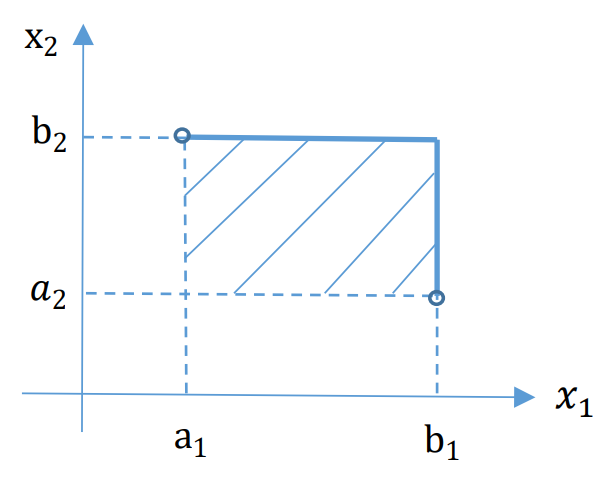
\includegraphics[scale=0.3]{img/f_example.png}
          \end{figure}


          В общем случае достаточно заметить, что 
          \[\bigtriangleup^i_{a_i,\,b_i}P(B_1\times\cdots\times B_{i - 1} \times (-\infty,\, x_i]\times\cdots\times B_n) = P(B_1\times\cdots\times(a_i,\,b_i]\times\cdots\times B_n)\]
	\end{enumerate}
\end{proof}

\begin{theorem}
  О построении вероятностной меры на $(\mathbb{R}^n,\, \mathcal{B}(\mathbb{R}^n))$ по функции распределения (б/д).

  Пусть $F(\vec{x})$ удовлетворяет всем свойствам из предыдущей леммы. Тогда $\exists!$ вероятностная мера на $(\mathbb{R}^n,\, \mathcal{B}(\mathbb{R}^n))$, для которой $F$ является функцией распределения.
\end{theorem}

\begin{definition}
  Пусть $P$ -- вероятностная мера на $(\mathbb{R}^\infty,\, \mathcal{B}(\mathbb{R}^\infty))$.

  $\forall n \in \mathbb{N}$ рассмотрим
  \[P_n(B) = P(F_n(B))\]
  где $F_n(B) = \{\vec{x} = (x_1,\,x_2,\,\cdots) :\: (x_1\,\,\cdots,\,x_n) \in B\}$ -- циллиндр с основанием $B$.

  Тогда $P_n$ будет вероятностной мерой в $\mathbb{R}^n$. Кроме того, $\forall n :\: \forall B \in \mathcal{B}(\mathbb{R}^n)$:
  \[P_n(B) = P_{n + 1}(B \times \mathbb{R})\]
  Это свойство согласованности.
\end{definition}

\begin{theorem}
  Колмогорова о мерах в $\mathbb{R}^\infty$ (б/д).

  Пусть $P_1,\,P_2,\,\cdots$ -- последовательность вероятностных мер в $\mathbb{R},\,\mathbb{R}^2,\,\cdots$, обладающая свойством согласованности.
  Тогда $\exists!$ вероятностная мера $P$ на $(\mathbb{R}^\infty,\,\mathcal{B}(\mathbb{R}^\infty))$, такая что 
  \[\forall n \in \mathbb{N} \: \forall B \in \mathcal{B}(\mathbb{R}^n):\: P_n(B) = P(F_n(B))\]
\end{theorem}

\section{Случайные элементы, случайные величины и векторы на вероятностном пространстве}
Пусть $(\Omega,\, \mathcal{F},\, P)$ -- вероятностное пространство, а $(E,\, \xi)$ -- измеримое пространство.

\begin{definition}
  Отображение $X:\: \Omega \to E$ называтся случайным элементом, если оно измеримо, то есть
  \[\forall B \in \xi:\: X^{-1}(B) = \{\omega :\: X(\omega) \in B\} \in \mathcal{F}\]
\end{definition}

\begin{definition}
  Если $(E,\, \xi) = (\mathbb{R},\, \mathcal{B}(\mathbb{R}))$, то случайный элемент называется случайной величиной.
\end{definition}

\begin{definition}
  Если $(E,\,\xi) = (\mathbb{R}^n,\, \mathcal{B}(\mathbb{R}^n))$, то случайный элемент называется случайным вектором.
\end{definition}

\begin{lemma}
  Критерий измеримости отображения.

  Пусть $\mathcal{M} \subset \mathcal{E}$, так чтобы $\sigma(\mathcal{M}) = \mathcal{E}$.
  Тогда $X:\: \Omega \to E$ является случайным элементом $\Leftrightarrow$
  \[\forall B \in \mathcal{M}:\: X^{-1}(B) \in \mathcal{F}\]
\end{lemma}

\begin{proof}
  $\Rightarrow$ очевидно.

  $\Leftarrow$ Рассмотрим
  \[\mathcal{D} = \{B \in \mathcal{E}:\: X^{-1}(B) \in \mathcal{F}\}\]
  Легко видеть, что $\mathcal{D}$ -- это $\sigma$-алгебра, так как $\mathcal{E}$ -- $\sigma$-алгебра, а прообраз сохраняет теоретико-множественные операции.

  По условию $\mathcal{M} \subset \mathcal{D} \Rightarrow \sigma(\mathcal{M}) = \mathcal{E} \subset \mathcal{D}$ в силу минимальности.
\end{proof}

\begin{corollary}
  Следующие утверждения эквивалентны:
  \begin{enumerate}
    \item $X:\: \Omega \to \mathbb{R}$ -- случайная величина
    \item $\forall x \in \mathbb{R}$:
    \[\{\omega:\: X(\omega) < x\} \in \mathcal{F}\]
    \item $\forall x \in \mathbb{R}$:
    \[\{\omega:\: X(\omega) \leq x\} \in \mathcal{F}\]
  \end{enumerate}
\end{corollary}

\begin{proof}
  Применяем лемму для $\mathcal{M} = \{(-\infty,\,x),\, x \in \mathbb{R}\}$ или $\mathcal{M} = \{(-\infty,\,x],\, x \in \mathbb{R}\}$. В обоих случаях $\sigma(\mathcal{M}) = \mathcal{B}(\mathbb{R})$
\end{proof}

\begin{corollary}
  $X := (X_1,\,\cdots,\,X_n):\: \Omega \to \mathbb{R}^n$ -- случайный вектор $\Leftrightarrow$
  \[\forall i = \overline{1,\,n}:\: X_i -- \text{ случайная величина}\]
\end{corollary}

\begin{proof}
  $\Rightarrow$ Пусть $B \in \mathcal{B}(\mathbb{R})$. Тогда 
  \[X_i^{-1}(B) = X^{-1}(\mathbb{R} \times\cdots\times \stackrel{i}{B}\times\cdots\times\mathbb{R}) \in \mathcal{F}\]
  Это верно, так как $X$ -- случайный вектор и 
  \[\mathbb{R} \times\cdots\times \stackrel{i}{B}\times\cdots\times \mathbb{R} \in \mathcal{B}(\mathbb{R}^n)\]
  $\Leftarrow$ Рассмотрим $\mathcal{M} = \{B_1\times\cdots\times B_n :\: B_i \in \mathcal{B}(\mathbb{R})\}$. Тогда $\sigma(\mathcal{M}) = \mathcal{B}(\mathbb{R}^n)$ и проверим условие леммы:
  \[X^{-1}(B_1\times\cdots\times B_n) = \stackrel{\in \mathcal{F}}{X^{-1}_1(B_1)} \cap\cdots\cap \stackrel{\in \mathcal{F}}{X_n^{-1}(B_n)} \in \mathcal{F}\]
  так как $\forall i = \overline{1,\,n}:\: X_i$ -- случайная величина.

  Значит по предыдущей лемме $\Rightarrow X$ -- случайный вектор.
\end{proof}

\section{Характеристики случайной величины и случайного вектора}
\begin{definition}
  Распределением случайной величины (вектора) $\xi$ называется вероятностная мера $P_\xi$ на $(\mathbb{R},\,\mathcal{B}(\mathbb{R}))$ ($(\mathbb{R}^n,\,\mathcal{B}(\mathbb{R}^n))$), определённая по правилу:
  \[P_\xi(B) = P(\xi \in B),\, B \in \mathcal{B}(\mathbb{R}) \; (\mathbb{R}^n)\]
\end{definition}

\begin{definition}
  Функцией распределения случайной величины $\xi$ называется
  \[F_\xi(x) = P(\xi \leq x) = P_\xi((-\infty,\, x])\]
\end{definition}

\begin{note}
  \[P(\xi_1 \leq x_1,\, \xi_2 \leq x_2) := P(\{\xi_1 \leq x_1\} \cap \{\xi_2 \leq x_2\})\]
\end{note}

\begin{definition}
  Если $\xi = (\xi_1,\,\cdots,\,\xi_n)$ -- случайный вектор, то его функцией распределения называется
  \[F_\xi(x_1,\,\cdots,\,x_n) = P_\xi((-\infty,\,x_1]\times\cdots\times (-\infty,\,x_n]) = P(\xi_1 \leq x_1,\, \cdots,\, \xi_n \leq x_n)\] 
\end{definition}

\begin{definition}
  Случайная величина является 
  \begin{itemize}
    \item Дискретной, если таково её распределение
    \item Абсолютно-непрерывной, если таково её распределение
    
    В этом случае $\xi$ имеет плотность $p_\xi(t) \geq 0$:
    \[F_\xi(x) = \int_{-\infty}^x p_\xi(t)dt\]
    \item Сингулярной, если таково её распределение
  \end{itemize}
\end{definition}

\begin{definition}
  Случайная величина $\xi$ называется простой, если она принимает конечное число значений. В этом случае $\xi$ имеет вид:
  \[\xi = \sum_{k = 1}^n x_k \mathbb{I}_{A_k}\]
  где $x_1,\,\cdots,\,x_n$ -- различные числа, $A_1,\,\cdots,\,A_n$ -- разбиение $\Omega$.
\end{definition}

\begin{definition}
  Пусть $\xi$ -- случайная величина (вектор) на $(\Omega,\, \mathcal{F},\,P)$. Сигма-алгеброй, порождённой $\xi$, называется 
  \[\mathcal{F}_\xi = \{\{\xi \in B\} :\: B \in \mathcal{B}(\mathbb{R})\} \: (\mathbb{R}^n)\]
  Заметим, что $\mathcal{F}_\xi \subset \mathcal{F}$
\end{definition}

\begin{definition}
  Случайная величина (вектор) $\eta$ является $\mathcal{F}_\xi$-измеримое, если $\mathcal{F}_\eta \subset \mathcal{F}_\xi$
\end{definition}

\begin{definition}
  Если $\xi$ -- это случайная величина, то положим
  \[\xi^+ := \max(\xi,\, 0);\;\;\; \xi^- := \max(-\xi,\, 0)\]
  Тогда, $\xi = \xi^+ - \xi^-$
\end{definition}

\begin{definition}
  Функция $\phi:\: \mathbb{R}^n \to \mathbb{R}^m$ называется борелевской, если 
  \[\forall B \in \mathcal{B}(\mathbb{R}^m) :\: \phi^{-1}(B) = \{x :\: \phi(x) \in B\} \in \mathcal{B}(\mathbb{R}^n)\]
\end{definition}

\begin{lemma} \label{BOREL_MEASURE}
  $\eta$ является $\mathcal{F}_\xi$-измеримой $\Leftrightarrow \exists$ борелевская функция $\phi$, такая что $\eta = \phi(\xi)$.
\end{lemma}

\begin{proof}
  $\Leftrightarrow$ Пусть $\eta = \phi(\xi)$ и $B \in \mathcal{B}(\mathbb{R})$. Тогда
  \[\{\eta \in B\} = \{\xi \in \stackrel{\in \mathcal{B}(\mathbb{R})}{\phi^{-1}(B)}\} \in \mathcal{F}_\xi \Rightarrow \mathcal{F}_\eta \subset \mathcal{F}_\xi\]
\end{proof}

\begin{theorem}
  О приближении простыми.
  
  \begin{enumerate}
    \item Пусть $\xi \geq 0$. Тогда $\exists$ последовательность $\mathcal{F}_\xi$-измеримых случайных величин $\{\xi_n,\, n \in \mathbb{N}\}$, такая что 
    \[0 \leq \xi_n \uparrow \xi\]
    \item Если $\xi$ -- произвольная случайная величина, то $\exists$ последовательность $\mathcal{F}_\xi$ измеримых простых случайных величин $\{\xi_n,\, n \in \mathbb{N}\}$, такая что
    \[\forall n \in \mathbb{N}:\: |\xi_n| \leq |\xi|,\, \lim_{n \to +\infty}\xi_n = \xi\]
  \end{enumerate}
\end{theorem}

\begin{proof}
  \begin{enumerate}
    \item Предъявим $\xi_n$ в явном виде:
    \[\xi_n = \sum_{k = 1}^{n2^n}\frac{k - 1}{2^n}\mathbb{I}_{\{\frac{k - 1}{2^n} \leq \xi < \frac{k}{2^n}\}}\]
    Легко видеть, что $0 \leq \xi_n \leq \xi_{n + 1}$ и $\xi = \lim\limits_{n \to +\infty} \xi_n$. Кроме того, $\forall n:\: \xi_n$ -- борелевская функция от $\xi \Rightarrow \xi_n$ -- по (\ref{BOREL_MEASURE}) это $\mathcal{F}_\xi$-измеримая случайная величина.
    \item Приближаем $\xi^+$ и $\xi^-$ по предыдущему пункту, затем берём разность
  \end{enumerate}
\end{proof}

\section{Независимости произвольного набора случайных величин}
\begin{definition}
  Случайные векторы $\{\xi_\alpha,\, \alpha \in \mathfrak{A}\}$ называются независимыми в совокупности, если независимы в совокупности порождённые ими $\sigma$-алгебры.
\end{definition}

\begin{corollary}
  Случайные векторы $\xi_1,\,\cdots,\,\xi_n,\, \xi_i \in \mathbb{R}^{k_i},\, i = \overline{1,\,n}$ независимы в совокупности $\Leftrightarrow$
  \[\forall B_1,\,\cdots,\,B_n \in \mathcal{B}(\mathbb{R}^{k_i}) :\: P(\xi_1 \in B_1,\,\cdots,\,\xi_n \in B_n) = \prod_{i = 1}^n P(\xi_i \in B_i)\]
\end{corollary}

\begin{lemma}
  Критерий независимости в терминах функций распределения

  Случайные величины $\xi_1,\,\cdots,\,\xi_n$ независимы в совокупности $\Leftrightarrow$
  \[\forall x_1,\,\cdots,\,x_n \in \mathbb{R} :\: P(\xi_1 \leq x_1,\,\cdots,\,\xi_n \leq x_n) = \prod_{i = 1}^n P(\xi_i \leq x_i)\]
  То есть функция распределения вектора распадается в произведение функций распределения компонент.
\end{lemma}

\begin{proof}
  $\Rightarrow$ очевидно из следствия выше.

  $\Leftarrow$ Проверим $\mathcal{M}_j = \{\{\xi_j \leq x\}:\: x \in \mathbb{R}\}$ -- подходящая $\pi$-система. Очевидно, что $\mathcal{M}_j$ -- это $\pi$-система и $\sigma(\mathcal{M}_j) \subset \mathcal{F}_{\xi_j}$.

  Тогда $\forall A \in \mathcal{M}_j$ имеет вид 
  \[A = \{\xi_j \in B\},\, B \in \mathcal{B}(\mathbb{R})\]
  Тогда введём
  \[\mathcal{D} := \{B \in \mathcal{B}(\mathbb{R}) :\: \{\xi_j \in B\} \in \sigma(\mathcal{M}_j)\}\]
  Тогда $\mathcal{D}$ -- это тоже $\sigma$-алгебра:
  \begin{enumerate}
    \item \[\{\xi_j \in \mathbb{R}\} = \Omega \in \sigma(\mathcal{M}_j) \Rightarrow \mathbb{R} \in \mathcal{D}\]
    \item \[\{\xi_j \in B_1 \cap B_2\} = \{\xi_j \in B_1\} \cap \{\xi_j \in B_2\} \in \sigma(\mathcal{M}_j) \Rightarrow B_1 \cap B_2 \in \mathcal{D}\]
    \item Аналогично
    \[B \in \mathcal{D} \Rightarrow \overline{B} \in \mathcal{D}\]
    \item Аналогично
    \[B_i \in \mathcal{D},\, i \in \mathbb{N} \Rightarrow \bigcup_{i = 1}^\infty B_i \in \mathcal{D}\]
  \end{enumerate}
  По построению все полуинтервалы $(-\infty,\, x] \in \mathcal{D} \Rightarrow \mathcal{B}(\mathbb{R}) \subset \mathcal{D}$. Значит, $\sigma(M_j) = \mathcal{F}_{\xi_j}$. Тогда, применяя (\ref{INDEPENDENCE_CRIT}), получим требуемое.
\end{proof}

\begin{note}
  То же самое верно и для случайных векторов.

  $\xi_1,\,\cdots,\,\xi_n$ независимы в совокупности $\Leftrightarrow$
  \[\forall \vec{x}_1,\,\cdots,\,\vec{x}_n :\: P(\xi_1 \leq \vec{x}_1,\,\cdots,\,\xi_n \leq \vec{x}_n) = \prod_{k = 1}^n P(\xi_1 \leq \vec{x}_1)\]
\end{note}

\begin{lemma}
  О независимости борелевских функций от независимых случайных величин.

  Пусть $\xi_1,\,\cdots,\,\xi_n$ -- независимые случайные векторы, $\xi_i \in \mathbb{R}^{k_i},\, k_i \in \mathbb{N},\, i = \overline{1,\,n}$. Пусть $f_i:\: \mathbb{R}^{k_i} \to \mathbb{R}^{m_i},\, i = \overline{1,\,n}$ -- борелевские функции. Положим $\eta_i = f_i(\xi_i)$. Тогда $\eta_1,\,\cdots,\,\eta_n$ -- независимые в совокупности.
\end{lemma}

\begin{proof}
  $\eta_1,\,\cdots,\,\eta_n$ независимы в совокупности $\Leftrightarrow \mathcal{F}_{\eta_1},\,\cdots,\,\mathcal{F}_{\eta_n}$ независимы в совокупности.

  Но $\mathcal{F}_{\eta_i} \subset \mathcal{F}_{\xi_i} \Rightarrow \mathcal{F}_{\eta_1},\,\cdots,\,\mathcal{F}_{\eta_n}$ независимы как подсистемы в независимых $\sigma$-алгебрах.
\end{proof}

\begin{corollary}
  $[\xi_1,\,\cdots,\,\xi_{n_1}],\, [\xi_{n_1 + 1},\,\cdots,\,\xi_{n_1 + n_2}],\,\cdots,\, [\xi_{n_1 + \cdots + n_{k - 1} + 1},\,\cdots,\, \xi_{n_1 + \cdots + n_k}]$ -- независимые блоки случайных величин. Пусть $f_j :\: \mathbb{R}^{n_j} \to \mathbb{R},\, j = \overline{1,\,k}$ -- борелевские функции. Тогда $f_1(\xi_1,\,\cdots,\,\xi_{n_1}),\, f_2(\xi_{n_1 + 1},\,\cdots,\,\xi_{n_1 + n_2}),\,\cdots,\, f_k(\xi_{n_1 + \cdots + n_{k - 1} + 1},\,\cdots,\, \xi_{n_1 + \cdots + n_k})$ -- независимые в совокупности случайные величины.
\end{corollary}

\begin{proof}
  Пускай $\eta_1 := (\xi_1,\,\cdots,\,\xi_{n_1}),\, \cdots,\, \eta_k := (\xi_{n_1 + \cdots + n_{k - 1} + 1},\,\cdots,\, \xi_{n_1 + \cdots + n_k})$. По предыдущей лемме $\eta_i,\, i = \overline{1,\,k}$ будут независимы в совокупности.
\end{proof}

\section{Теорема о математическом ожидании произведения независимых случайных величин с конечными математическими ожиданиями}
\begin{theorem}
  О математическом ожидании произведения независимых случайных величин с конечными математическими ожиданиями.

  Пусть $\xi,\, \eta$ -- независимые случайные величины, $E\xi,\, E\eta$ -- конечные. Тогда $E\xi\eta$ тоже конечно, причём $E\xi\eta = E\xi\cdot E\eta$.
\end{theorem}

\begin{proof}
  Пусть сначала $\xi,\, \eta$ -- простые случайные величины, то есть
  \[\xi = \sum_{i = 1}^n x_i\mathbb{I}\{\xi = x_i\};\; \eta = \sum_{j = 1}^m y_j\mathbb{I}\{\eta = y_j\}\]
  где $x_1,\,\cdots,\,x_n$ -- значения $\xi$, а $y_1,\,\cdots,\,y_j$ -- значения $\eta$. Тогда
  \[\xi\eta = \sum_{i = 1}^n\sum_{j = 1}^m x_iy_j \mathbb{I}\{\xi = x_i,\, \eta = y_j\}\]
  Берём $E$ от обеих частей:
  \begin{align*}
    E\xi\eta = \sum_{i = 1}^n\sum_{j = 1}^m x_iy_j P(\xi = x_i,\, \eta = y_j) \stackrel{\independent}{=} \sum_{i = 1}^n\sum_{j = 1}^m x_iy_j P(\xi = x_i)P(\eta = y_j) = \\
    \left(\sum_{i = 1}x_iP(\xi = x_i)\right)\left(\sum_{j = 1}^my_jP(\eta = y_j)\right) = E\xi\cdot E\eta
  \end{align*}
  Далее, пусть $\xi,\,\eta \geq 0$ -- неотрицательные случайные величины. Тогда рассмотрим последовательности простых случайных величин $\{\xi_n,\, n \in \mathbb{N}\},\, \{\eta_m,\, m \in \mathbb{N}\}$, такие что
  \[0 \leq \xi_n \uparrow \xi ;\;\;\; 0 \leq \eta_m \uparrow \eta\]
  и $\forall n \in \mathbb{N}:\: \xi_n$ является $\mathcal{F}_\xi$-измеримой, $\eta_n$ -- $\mathcal{F}_\eta$-измеримой.

  Следовательно, $0 \leq \xi_n\eta_n \uparrow \xi\eta$ и $\forall n \in \mathbb{N}:\: \xi_n \independent \eta_n$. По определению мат. ожидания:
  \[E\xi\eta = \lim_{n \to +\infty} E\xi_n\eta_n \stackrel{\independent}{=} \lim_{n \to +\infty}E\xi_n\cdot \lim_{n \to +\infty}E\eta_n = E\xi\cdot E\eta\]
  Теперь пусть $\xi,\, \eta$ -- произвольные случайные величины. Тогда $\xi^\pm \independent \eta^\pm$, как функции от независимых случайных величин. Причём
  \[(\xi\eta)^+ = \xi^+\eta^+ + \xi^-\eta^- ;\;\;\; (\xi\eta)^- = \xi^+\eta^- + \xi^-\eta^+\]
  По определению
  \begin{align*}
    E\xi\eta = E(\xi\eta)^+ - E(\xi\eta)^- = E\xi^+\eta^+ + E\xi^-\eta^- - E\xi^+\eta^- - E\xi^-\eta^+ \stackrel{\independent}{=} \\
    E\xi^+\cdot E\eta^+ + E\xi^-\cdot E\eta^- - E\xi^+ \cdot E\eta^- - E\xi^-\cdot E\eta^+ = (E\xi^+ - E\xi^-)(E\eta^+ - E\eta^-) = \\
    E\xi \cdot E\eta
  \end{align*}
\end{proof}

\section{Теорема о замене переменных в интеграле Лебега...}
\begin{theorem}
  О замене переменных в интеграле Лебега.

  Пусть $\xi$ -- случайный вектор из $\mathbb{R}^m$ на $(\Omega,\, \mathcal{F},\,P),\, P_\xi$ -- его распределение. Тогда $\forall g:\: \mathbb{R}^m \to \mathbb{R}$ -- борелевской функции, выполнено
  \[Eg(\xi) = \int_\Omega g(\xi)dP = \int_{\mathbb{R}^m}g(x)P_\xi(dx)\]
\end{theorem}

\begin{proof}
  Пусть сначала $g(x) = \mathbb{I}_A(x)$, где $A \in \mathcal{B}(\mathbb{R}^m)$. Тогда 
  \[
    Eg(\xi) = E\mathbb{I}\{\xi \in A\} = P(\xi \in A) = P_\xi(A) = \int_A P_\xi(dx) = \int_{\mathbb{R}^m}\mathbb{I}_A(x)P_\xi(dx) = \int_{\mathbb{R}^m}g(x)P_\xi(dx)
  \]
  В формуле из утверждения теоремы обе части линейны по $g$. Равенство верно для индикаторов $\Rightarrow$ верно для простых функций.

  Если $g \geq 0$, то рассмотрим последовательность простых функций $0 \leq g_n \uparrow g$. Тогда 
  \[\int_{\mathbb{R}^m}g(x)P_\xi(dx) \stackrel{n \to +\infty}{\leftarrow} \int_{\mathbb{R}^m}g_n(x)P_\xi(dx) = Eg_n(\xi) \stackrel{n \to +\infty}{\to} Eg(\xi)\]
  для неотрицательных доказали.

  Если $g$ -- произвольная функция, то раскладываем $g = g^+ - g^-$ и пользуемся линейностью.

  Причём все математические ожидания будут конечны, бесконечны и неопределены одновременно.
\end{proof}

\begin{corollary}
  \begin{enumerate}
    \item Для вычисления $Eg(\xi)$ достаточно знать распределение $P_\xi$.
    \item Если распределение $\xi,\, \eta$ совпадают, то $\forall$ борелевской функции $g(x)$ выполнено
    \[Eg(\xi) = Eg(\eta)\]
    \item Если $\xi$ -- случайная величина, то
    \[E\xi = \int_\mathbb{R} xP_\xi(dx)\]
  \end{enumerate}
\end{corollary}

\begin{note}
  \[dF(x) := P(dx)\]
  где $F$ -- функция распределения вероятностной меры $P$.
\end{note}

\begin{definition}
  Пусть $P$ -- вероятностная мера на $(\mathbb{R}^m,\, \mathcal{B}(\mathbb{R}^m))$, $\mu$ -- $\sigma$-конечная мера на $(\mathbb{R}^m,\, \mathcal{B}(\mathbb{R}^m))$. Мера $P$ имеет плотность $p(t) \geq 0$ по мере $\mu$, если 
  \[\forall B \in \mathcal{B}(\mathbb{R}^m) :\: P(B) = \int_B p(t)\mu(dt)\]
\end{definition}

\begin{theorem}
  О плотности.
  
  Пусть случайный вектор $\xi \in \mathbb{R}^m$ имеет распределение $P_\xi$, и $P_\xi$ имеет плотность $p(t)$ по $\sigma$-конечной мере на $(\mathbb{R}^m,\, \mathcal{B}(\mathbb{R}^m))$. Тогда $\forall$ борелевской функции $g(x) :\: \mathbb{R}^m \to \mathbb{R}$ выполнено
  \[Eg(\xi) = \int_{\mathbb{R}^m}g(x)P_\xi(dx) = \int_{\mathbb{R}^m}g(x)p(x)\mu(dx)\]
\end{theorem}

\begin{proof}
  Пусть сначала $g(x) = \mathbb{I}_A(x)$, где $A \in \mathcal{B}(\mathbb{R}^m)$. Тогда 
  \[
    Eg(\xi) = P(\xi \in A) = P_\xi(A) = \int_Ap(x)\mu(dx) = \int_{\mathbb{R}^m}\mathbb{I}_A(x)p(x)\mu(dx) = \int_{\mathbb{R}^m}g(x)p(x)\mu(dx)
  \]
  Обе части доказываемого равенства линейны по $g \Rightarrow$ формула верна для простых функций.

  Если $g \geq 0$, то рассмотрим последовательность простых функций $\{g_n,\, n \in \mathbb{N}\}$, такую что $0 \leq g_n(x) \uparrow g(x)$. Тогда по определению интеграла Лебега:
  \[
    Eg(\xi) = \lim_{n \to +\infty}Eg_n(\xi) = \lim_{n \to +\infty} \int_{\mathbb{R}^m}g_n(x)p(x)\mu(dx) = \int_{\mathbb{R}^m}g(x)p(x)\mu(dx)
  \]
  (по теореме о монотонной сходимости)

  Для произвольной $g$ раскладываем $g(x) = g^+ - g^-$ и пользуемся линейностью.
\end{proof}

\begin{corollary}
  Пусть $\xi$ -- дискретная случайная величина, сосредоточенная на $X$. Тогда
  \[Eg(\xi) = \sum_{x \in X}g(x)P(\xi = x)\]
\end{corollary}

\begin{proof}
  Мы знаем, что $p(x) = P_\xi(\{x\}) = P(\xi = x)$. Тогда
  \[Eg(\xi) = \int_\mathbb{R}g(x)p(x)\mu(dx) = \sum_{x \in X} g(x)P(\xi = x)\]
\end{proof}

\begin{corollary}
  Пусть $\xi$ -- абсолютно непрерывная случайная величина с плотностью $p(x)$. Тогда
  \[Eg(\xi) = \int_\mathbb{R} g(x)p(x)dx\]
\end{corollary}

\begin{corollary}
  Пусть $\xi$ -- случайный вектор из $\mathbb{R}^m$ с плотностью $p(x)$. Тогда
  \[Eg(\xi) = \int_{\mathbb{R}^m}g(\vec{x})p(\vec{x})d\vec{x}\]
\end{corollary}

\end{document}
